%
%  cribsheet.tex
%  midterm-study-guide
%
%  Created by Illya Starikov on 10/20/17.
%  Copyright 2017. Illya Starikov. All rights reserved.
%

\RequirePackage[l2tabu, orthodox]{nag}
\documentclass[12pt]{scrartcl}

\usepackage{amssymb,amsmath,verbatim,graphicx,microtype,upquote,units,booktabs,akkwidepage}

\newcommand{\chapterNumber}[1]{
    \setcounter{section}{#1}
    \addtocounter{section}{-1}
}
\title{Final Cribsheet}

\usepackage{graphicx,forest,tikz-qtree,graphics}
\date{\today}
\let\oldemptyset\emptyset{}
\let\emptyset\varnothing{}
\newcommand{\cost}[1]{\text{cost}\left(#1\right)}

\begin{document}
\maketitle

\section{Recursion}
\begin{itemize}
    \item A program is \textbf{recursive} if it calls or refers to itself.

    \item The structure of recursion is as follows:
\end{itemize}

\begin{lstlisting}
    if CONDITION:
        DIRECT CASE
    else:
        RECURSIVE CASE
\end{lstlisting}

\begin{itemize}
    \item The 3--5 problem is as follows:
\end{itemize}

\begin{lstlisting}
def f35(n):
    if n < 8:
        return "Error"
    elif n == 8:
        return (1, 1)
    elif n == 9:
        return (3, 0)
    elif n == 10:
        return (0,2)
    else:
        m3, m5 = f35(n - 3)
        return (1 + m3, m5)
\end{lstlisting}

\begin{itemize}
    \item Recursive Insertion Sort is as follows:
\end{itemize}

\begin{lstlisting}
def InsSortR(L):
    if len(L) < 2:
        return L
    else:
        return Insert(L[-1], InsSortR(L[:-1]))

def Insert(e,sL):
    if 0 == len(sL):
        return [e]
    elif (e >= sL[-1]):
        return sL+[e]
    else:
        return Insert(e, sL[:-1]) + [sL[-1]]
\end{lstlisting}

\begin{itemize}
    \item Euclid's Elements is the most important book ever published.
        \begin{itemize}
            \item It laid the foundations for modern mathematics and science.
        \end{itemize}

    \item \shellcmd{GCD} can be defined as follows
\end{itemize}

\begin{lstlisting}
def GCD(a, b):
    if (a % b == 0):
        return b

    return GCD(b, a % b)
\end{lstlisting}

\section{Recursion Part II}
\begin{itemize}
    \item The Tower of Hanoi has runtime $2^n - 1$.
\end{itemize}

\begin{lstlisting}
def H(n,a,b):
    if n == 0:
        return []
    if x == y:
        return []

    m = otherNeedle(x, y)
    return Hanoi(n - 1, x, m) + [(n, x, y)] + Hanoi(n - 1, m, y)

    def otherNeedle(n1,n2):
        if n1 == n2:
            return "ERROR -- Two needles are the same!"
            J = ['A','B','C']

        J.remove(n1)
        J.remove(n2)
        return J[0]
\end{lstlisting}

\begin{itemize}
    \item To generate anagrams:
\end{itemize}

\begin{lstlisting}
def anagram(st):
    if st == '':
        return ['']

    lout =[]
    for i in range(len(st)):
        st2 = st[:i] + st[i+1:]
        lout2 = anagram(st2)

        for w in lout2:
            lout.append(st[i]+w)
            return lout
\end{lstlisting}

\section{Proof by Recursion}
\begin{itemize}
    \item A \textbf{property $P$ on a domain $D$} is a function $D$ that accepts inputs from the domain $D$ and return a Boolean value. If $P$ is a property on $D$, and $d$ is in $D$, then we say that \textbf{$P$ holds for $d$} if $P(d)$ is true. Similarly, \textbf{$P$ does not hold for $d$} if $P(d)$ is false.

    \item The proof by recursion has the following steps:

        \begin{description}
            \item[Define the Problem] Clearly state the objects you are dealing with, provide names and definitions for all functions you are talking about, clearly state what you are trying to prove.
            \item[Check the Stopping Values + Two More] Checking that whatever you are tying to prove is required for the stopping value, but optional for two other values.
            \item[Check that the Recursion Stays in $D$] Prove that if recursion in $P$ is triggered by values in $D$, then the values in the call are also in $D$.
            \item[Check That Recursion Halts] We use the \textbf{counting strategy}: assign a \textbf{non-negative} integer as a counter to every value in the domain $D$. If whenever recursion is triggered, the counter associated with called values are $<$ the value associate with the calling value, recursion will halt!
            \item[Check Inheritance] You may assume that $P$ is true for all values called recursively; however, you must then prove that $P$ holds for the calling value.
            \item[Conclude the Proof] Invoke the Principle of Recursion.
        \end{description}
\end{itemize}

\section{Induction}
\begin{itemize}
    \item Some notes on The Modulus (\%)
        \begin{itemize}
            \item $P \% Q$ is always between $0$ and $Q - 1$.
            \item $(P + R) \% Q = (P \% Q + R \% Q) \% Q$
            \item $P = S \times Q + P \% Q$.
            \item $(P \times R) \% Q = (P \% Q) \times (R \% Q)$
        \end{itemize}

    \item Mathematical induction is like recursion except that:
        \begin{itemize}
            \item Uses predicates vs.\ recursive program
            \item The domain is always a set of \textbf{integers}.
        \end{itemize}

    \item Proof by simple induction has the following steps:
        \begin{description}
            \item[Define the problem] Clearly define the domain $D$, which must be of the form $D = s \ldots \infty$.
            \item[Check Base Case \& Two Other Values]
            \item[Prove for all $n > s$, that if $P(n - 1)$ is true, then $P(n)$ is true]
            \item[Conclude the proof]
        \end{description}

    \item The principle of well-ordering is as follows

        \begin{quote}
            Every non-empty set of natural numbers has at least one element.
        \end{quote}

    \item To Euclid, \textbf{axioms} are statements that are true in all domains. Postulates are statements that are true in some domain.
    \item Via Peano's postulates, there is a set called $N$ consisting of objects we call ``numbers''. There is also a operation of \textit{successor} denoted by $*$ from $N$ into $N$.
        \begin{enumerate}
            \item There is an objected called $0$.
            \item For all $p$, $p* \neq 0$
            \item If $p*$ = $q*$, then $p = q$.
            \item If $Q$ is a subset of $N$, such that

                \begin{itemize}
                    \item $0$ is in $Q$
                    \item If $q$ in $Q$, then $q*$ in $Q$
                    \item Then $Q = N$
                \end{itemize}
        \end{enumerate}
\end{itemize}

\section{Big Oh Algorithms}
\begin{description}
    \item[Big-O] $O(g(n)) = \{ f(n) : \ \text{there exists positive constant $c$ and $n_0$ such that} \ 0 \leq f(n) \leq c \ g(n) \ \text{for all} \ n \geq n_0 \}$
    \item[Big-$\Omega$] $\Omega(g(n)) = \{ f(n) : \ \text{there exists positive constants $c$ and $n_0$ such that} \ 0 \leq c \ g(n) \leq f(n) \ \text{for all} \ n \geq n_0 \}$
    \item[Big-$\Theta$] $\Theta(g(n)) = \{ f(n) : \ \text{there exists positive constants $c_1, c_2$ and $n_0$ such that} \\ \ 0 \leq c_1 \ g(n) \leq f(n) \leq c_2\ g(n) \ \text{for all} \ n \geq n_0 \}$
\end{description}

\begin{itemize}
    \item A loop invariant needs to satisfy $3$ conditions:

        \begin{description}
            \item[Initilization] Must be correct before the loop begins.
            \item[Maintenance] Each iteration maintains loop property.
            \item[Termination] Property holds when loop terminates.
        \end{description}
\end{itemize}

\begin{description}
    \item[Incremental Improvement] Improve things one step at a time.
    \item[Divide and Conquer] Divide the problem into a number of subproblems that are instances of the same problem and put your solution together from the sub-solutions.
\end{description}

\section{Fibonacci Numbers, Sums, and Series}
\begin{itemize}
    \item The Fibonacci numbers are defined as follows:

        \begin{equation*}
            F_n = \begin{cases}
                0 & \Leftrightarrow n = 0 \\
                1 & \Leftrightarrow n = 1 \\
                F_{n-1} + F_{n - 2} & \Leftrightarrow n > 1
            \end{cases}
        \end{equation*}

    \item A \textit{sequence} is a function $f: \mathbb{N} \rightarrow \mathbb{R}$ where we denote $f(n)$ by $a_n$.
    \item A \textit{series} is a sequence $S_n$ associated with another sequence $a_n$ such that $S_n = \sum _{k = 0} ^n a_k$.
    \item Given a sequence we will refer to the partial sums as the \textit{associated series}.
    \item A \textit{arithmetic progression} is a series where each term in the associated sequence differs from the preceding term by a constant.
    \item A \textit{geometric progression} is a series were each term in the associated sequence is a constant multiple of the preceding term.
    \item The harmonic series is defined as

        \begin{equation*}
            H_n = \sum _{k = 1} ^n \frac{1}{k}
        \end{equation*}

    \item If $f$ is monotonically increasing, then

        \begin{equation*}
            \int_{m - 1} ^n f(x)\, dx \leq
            \sum_{k = m} ^n f(k) \leq
            \int_m ^{n + 1} f(x)\, dx
        \end{equation*}


    \item If $f$ is monotonically decreasing, then

        \begin{equation*}
            \int_{m - 1} ^n f(x)\, dx \geq
            \sum_{k = m} ^n f(k) \geq
            \int_m ^{n + 1} f(x)\, dx
        \end{equation*}

    \item for $|r| < 1$,

        \begin{equation*}
            S = \sum _{k = 0} ^\infty r^k = \frac{1}{1 - r}
        \end{equation*}
\end{itemize}

\section{Disjoint Sets}
\begin{itemize}
    \item For all equivalence relations, $a\,R\,b$ and $b\,R\,c \implies a\,R\,c$, so once there is an intersection between two blocks in a partition, those blocks need to be joined into a single block.
\end{itemize}

\begin{equation*}
    \prod _{k = 1} ^n 2^k = 2^{\sum_{k = 1} ^n k} = 2^{\frac{n(n + 1)}{2}}
\end{equation*}

\begin{itemize}
    \item We can approximate $n$! by

        \begin{equation*}
            n! \approx \sqrt{2\pi n} {\left( \frac{n}{e} \right)}^n
        \end{equation*}

    \item Sterling's Formula is as follows:

        \begin{equation}
            \int _1 ^n \ln x\, dx \leq \sum_{k = 2} ^n \ln k \leq \int _2 ^{n + 1} \ln x\, dx
        \end{equation}

    \item A set is a collection of objects.
    \item Some commons sets are:
        \begin{description}
            \item[$\emptyset{}$] The Empty Set
            \item[$\mathbb{N}$] The natural numbers
            \item[$\mathbb{Z}$] The integers
            \item[$\mathbb{Q}$] The rational numbers
            \item[$\mathbb{R}$] The real numbers
            \item The set of all finite graphs
            \item The set of all finite trees
            \item The set of all strings
        \end{description}

    \item DeMorgan's Laws

        \begin{equation*}
            (A \cap B)' = A' \cup B' \qquad (A \cup B)' = A' \cup B'
        \end{equation*}

    \item Absorption Laws

        \begin{equation*}
            A \cap (A \cup B) = A \qquad A \cup (A \cap B) = A
        \end{equation*}

    \item $R$ is \textbf{reflexive} iff $\forall a \in A$, $a\, R\, a$, which means $(a, a) \in R$.
    \item $R$ is \textbf{symmetric} iff $\forall a, b \in A$, $a\, R\, b \equiv b\, R\, a$.
    \item $R$ is \textbf{antisymmetric} iff $\forall a, b \in A$, $a\, R\, b$ and $b\, R\, a \rightarrow a = b$.
    \item $R$ is \textbf{transitive} iff $\forall a, b, c \in A$ and $a\, R\, b$, $a\, R\, b \rightarrow a\, R\, b$.
    \item $R$ is an \textbf{equivalence relation} iff it is reflexive, symmetric and transitive.
    \item $R$ is a \textbf{partial order} iff it is reflexive, antisymmetric and transitive.
    \item $R$ is a \textbf{total order} iff it is a partial order such that $\forall a, b \in A$ either $a\, R\, b$ or $b\, R\, a$.
\end{itemize}

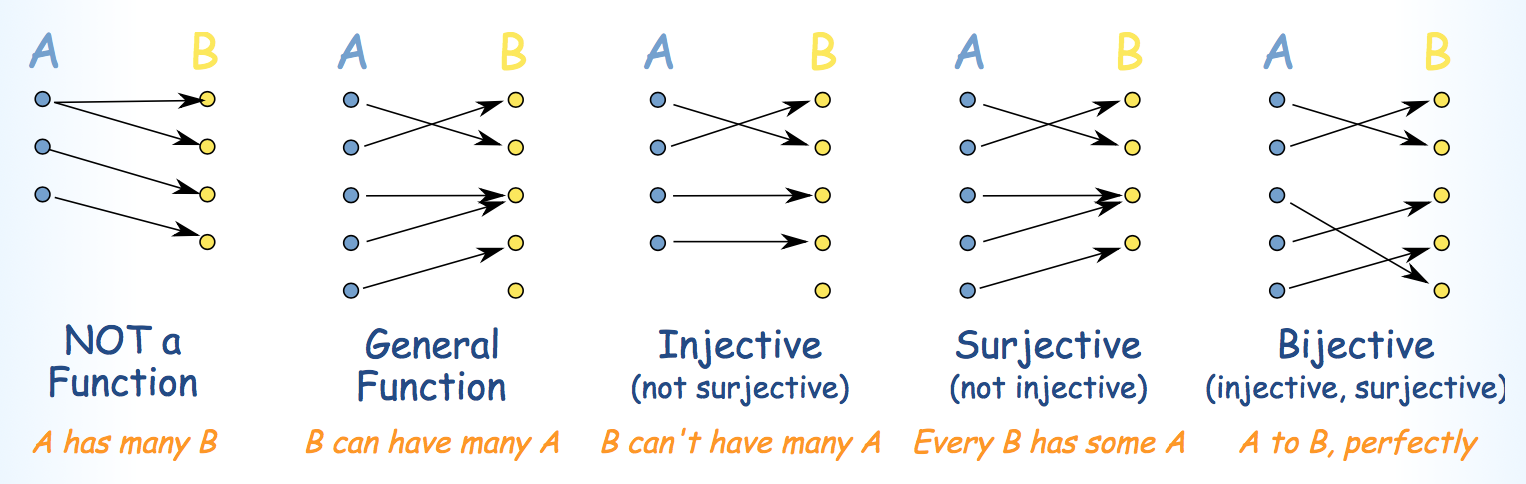
\includegraphics[width=\textwidth]{./assets/injective-etc.png}


\section{Graph Theory I}
\begin{itemize}
    \item Let $P$ be a path of length $K > 0$ and let $i,j \in range(k+1) \mid P(i) = P(j)$. We define $Trim(p,i,j)$ to be a function $g: k + i - j + 1 \rightarrow \mathbb{V}$.
    \item Let $p$ and $q$ be paths in a graph $G$. $q$ is said to be \textbf{reduction} of $p$ iff $q$ can be derived from $p$ by a finite number of trimming operations.
    \item The set of all paths that can be obtained by applying finite sequences of trimming operations to $p$ is called the set of \textbf{reduced path of $p$} or \textbf{reductions of $p$}
    \item In a finite graph with even a single edge, the number of paths is infinite.
    \item We call the equivalence classes of $R$ the \textbf{connected components} of $G$.
    \item A \textbf{cycle} is a path of length $\geq 3$ that begins and ends at the same vertex --- \textit{self-loops are not allowed in graphs}.
    \item A \textbf{simple cycle} is a cycle that has no repetition of vertices except for the first and last vertex.
    \item A simple cycle is not a simple path.
    \item If there are two different simple paths between $a$ and $b$ in a graph, $G$, then there is a simple cycle in $G$.
    \item A \textbf{simple path} is a path such that no vertex appears more than once. (if $f : $\underbar{$n$}$\rightarrow \mathbb{V}$ it's an \textit{injection})
    \item If $\exists P = (a,\ldots, b)$, then $b$ is \textbf{Reachable}  from $a$

        \begin{itemize}
            \item let $R$ be the relation on $\mathbb{V} \iff b$ is reachable from $a$.
            \item $R$ is \textit{reflexive}: $aRa$ given by $f(0) = a$
            \item $R$ is \textit{symmetric}: $aRb \to bRa$ given by \textit{Reverse Paths}
            \item $R$ is \textit{transitive}: $aRb, bRc \to aRc$ given by \textit{Path Concatenation}
            \item Equivalence Classes of $R$ are all the connected Components of a graph $G$.
        \end{itemize}

    \item A graph is \textbf{acyclic} iff it does not contain simple cycles.
    \item Two graphs $G_1 = (V_1, E_1)$ and $G_2 = (V_2, E_2)$ are said to be \textbf{isomorphic} iff there is a bijection $f: V_1 \rightarrow V_2$ such that $\{a, b\} \in E_1$ iff $\{f(a), f(b)\} \in E_2$.
        \begin{itemize}
            \item Basically, if the graphs are the same.
        \end{itemize}

    \item No Euler path is possible if there are more than $2$ odd degree vertices.
        \begin{itemize}
            \item The converse is also true, there exists an Euler path if a graph has $2$ or $0$ vertices of odd degree.
        \end{itemize}
\end{itemize}


\section{Euler's Formula (Digraphs)}
\begin{itemize}
    \item For a planar connected graph, we have

        \begin{equation*}
            V - E + F = 2
        \end{equation*}

    \item True for closed shapes because $E = V$ and $F = 2$.
    \item For any planar graph with $V \geq 3$, we must have $E \leq 3V - 6$.
    \item As a result of Euler's Formula,
        \begin{itemize}
            \item $K_3$ is not planar.
            \item $K_{3,\, 3}$ is not planar.
            \item There are only 5 regular solids.
            \item A soccer ball must have exactly \num{12} pentagon
        \end{itemize}

    \item Any planar graph has a vertex of degree $\leq 5$.
\end{itemize}


\section{Graph Theory II}
\begin{itemize}
    \item If $G = (V,\, E)$ is an undirected graph, then $\sum _{v \in V} \deg(v) = 2|E|$.
    \item A planar graph is a graph that can be drawn in the plane without having any lines cross.
\end{itemize}


\section{Master Theorem \& Fast Multiplication}
\begin{theorem}
Let $a \geq 1$ and $b > 1$ be constants, let $f(n)$ be a function, and let $T(n)$ be defined on the non-negative numbers by the recurrence

\begin{equation}\label{eq:recurrence}
    T(n) = a\, T(\nicefrac{n}{b}) + f(n)
\end{equation}

\noindent where we interpret $\nicefrac{n}{b}$ to mean either $\floor*{\nicefrac{n}{b}}$ or $\ceil*{\nicefrac{n}{b}}$. Then $T(n)$ has the following asymptotic bounds:

\begin{enumerate}
    \item If $f(n) = \bigO{n^{\log_b a - \epsilon}} $ for some constant $\epsilon > 0$, then $T(n) = \bigTheta{n^{\log _b a}}$.
    \item If $f(n) = \bigTheta{n^{\log_b a}} $, then $T(n) = \bigTheta{n^{\log _b a} \lg n}$.
    \item If $f(n) = \bigOmega{n^{\log_b a + \epsilon}} $ for some constant $\epsilon > 0$, and if
        \begin{equation*}
            a\, f(\nicefrac{n}{b}) < c\, f(n)
        \end{equation*}

    for some constant $c < 1$ and sufficiently large $n$, then $T(n) = \bigTheta{f(n)}$.
\end{enumerate}
\end{theorem}

\begin{itemize}
    \item To use the substitution method,
        \begin{enumerate}
            \item Guess the form of the solution
            \item Use Mathematical Induction to find the constants and show that the solutions works
        \end{enumerate}
    \item The sum of two homogeneous solutions is a homogeneous solution
    \item Multiplying a homogeneous solution by a constant gives a homogeneous solution
    \item The linear combination of homogeneous solutions is a homogeneous solution
    \item For the Fibonacci recursion
        \begin{equation*}
            F_n + F_{n - 1} - F_{n - 2} = 0
        \end{equation*}

    \item The associated equations is $x^2 - x - 1 = 0$, which has the roots $\frac{1 \pm \sqrt{5}}{2}$.
        \begin{itemize}
            \item Note that $\frac{1 + \sqrt{5}}{2}$ the golden ration $\phi$.
        \end{itemize}
\end{itemize}


\section{Graphs \& Trees}
\begin{itemize}
    \item A digraph $(V, A)$ is \textbf{bipartite digraph} iff we can write $V = B \cup C$, where $B \cap C = \emptyset$ and all arcs have their tails in $B$ and their heads in $C$.
    \item A \textbf{forest} is an acyclic graph
    \item A \textbf{free tree} is an acyclic, connected graph
    \item A \textbf{DAG} is a directed, acyclic graph
    \item A \textbf{rooted tree} is a triple $(V, E, r)$ where $(V, E)$ is a free tree and $r \in V$ is a distinguished vertex called the \textbf{root}.
    \item We say that $a$ is \textbf{proper ancestor} of $b$ iff $a$ is an ancestor of $b$, but $a \neq b$.
    \item We say that $a$ is \textbf{proper descendant} of $a$ iff $b$ is an ancestor of $a$, but $a \neq b$.
    \item A \textbf{positional tree} is an ordered tree where the children are labeled by distinct positive integers
    \item A \textbf{$k$-ary} tree is a positional tree where the labels are $\leq k$.
    \item A \textbf{complete $k$-ary} tree is a $k$-ary tree where each non-leaf node has all $k$ children and all leaves have the same depth.
    \item $G = (V, E)$. The following are equivalent.
        \begin{itemize}
            \item $G$ is a free tree (connected and acyclic).
            \item Any two vertices in $G$ are connected by a unique simple path.
            \item $G$ is connected, but removing any edge disconnects $G$
            \item $G$ is connected and $|E| = |V| - 1$.
            \item $G$ is a acyclic and $|E| = |V| - 1$
            \item $G$ is acyclic but adding any edge creates a cycle.
        \end{itemize}

    \item If $G$ is connected then $|E| \geq |V| - 1$.
\end{itemize}

\section{Disjoint Set Graph Algorithms}
\begin{lstlisting}
DFS(G)
for each vertex $u \in G.V$
    u.color = WHITE
    u.$\pi$ = NIL

time = 0
for each vertex $u \in G.V$
    if u.color == WHITE
        DFS-VISIT(g, u)

DFS-VISIT(G, u)
time = time + 1
u.d = time
u.color = GRAY

for each $v \in G.Adj[u]$
    if v.color == WHITE
        v.$\pi$ = u
        DFS-VISIT(g, v)

u.color = BLACK
time = time + 1
u.f = time
\end{lstlisting}

\begin{lstlisting}
BFS(G,s)
for each vertex $u \in G.V - \{ s \}$
    u.colors = WHITE
    u.d = $\infty$
    u.$\pi$ = NIL

s.color = gray
s.d = 0
s.$\pi$ = NIL
Q = $\emptyset$

ENQUEUE(Q, s)
while Q $\neq \emptyset$
    u = DEQUEUE(Q)

    for each $v \in G.Adj[u]$
        if v.color == WHITE
            v.color = GRAY
            v.d = u.d + 1
            v.$\pi$ = u
            ENQUEUE(Q, v)
    u.color = BLACK
\end{lstlisting}

\section{Disjoint Sets Graph Algorithms II}
\begin{itemize}
    \item To topologically sorting a $DAG$
        \begin{enumerate}
            \item Apply \texttt{DFS} to the digraph $D$
            \item As each node finishes, put it at the beginning of the list
            \item Return the list
        \end{enumerate}
\end{itemize}

\section{Probability}
\begin{itemize}
    \item Using set notation, a \textit{Sample Space} is a set.
    \item An event is just a subset of a sample space $S$
    \item An \textbf{elementary} is just a point in the sample space $S$.
    \item A \textbf{certain event} is just $S$
    \item A \textbf{null event} is just $\emptyset$
    \item Two events are \textbf{mutually exclusive} iff their intersection is $\emptyset$
    \item Nothing is random about sample spaces and events.
    \item A \textbf{discrete probability distribution} on a sample space $S$ is just a function $f : S \rightarrow \mathbb{R}$
        \begin{enumerate}
            \item $f(x) \geq 0, \forall x \in S$
            \item $\sum _{x \in S} f(x) = 1$
        \end{enumerate}

    \item A \textbf{probability space} is a pair $(S, f)$, where is a $S$ is a sample space and $f$ is a probability distribution on $S$.
    \item Given a probability space $(S, f)$ and $E \subset S$ an event, the \textbf{probability} of $E$ is denoted $\Pr(E) = \sum _{x \in E} f(x)$
    \item The \textbf{uniform distribution} is defined for \textit{finite} sample spaces as follows:
        \begin{itemize}
            \item $f : S \rightarrow \mathbb{R}$ is given by $f(x) = \frac{1}{|S|} \forall x \in S$
            \item Usually assume uniform distribution unless have other evidence
        \end{itemize}

    \item The normal distribution is a distribution over the reals, $\mathbb{R}$, so we will not use it much.
    \item The \textbf{conditional probability of $A$ given $B$} denoted $\Pr(A | B)$ is \textbf{defined} as $\frac{\Pr(A \cap B)}{\Pr(B)}$
    \item Bayes's Theorem is as follows:

        \begin{equation*}
            \Pr(A|B) = \frac{\Pr(A) \Pr(B | A)}{\Pr(B)}
        \end{equation*}

    \item A \textbf{random variable} is a function from a sample space into the real numbers.
    \item The \textbf{density probability function} of $X$, written $f_x (r) = \Pr(X^{-1}(r)) \forall r \in \mathbb{R}$.
    \item The \textbf{expected value of random variable $V$}, $E(V)$, is defined by

        \begin{equation*}
            E(V) = \sum _{x \in S} V(x) \Pr(\{ x \})
        \end{equation*}

        This is just the average value of $V$.

    \item For all probability spaces and random variables, $\min \left\{ V(x) | x \in S \right\} \leq E(V) \leq \max \left\{ V(x) | x \in S \right\}$
\end{itemize}


\section{Probability II}
\begin{itemize}
    \item Chebychev's theorem is as follows

        \begin{equation*}
            \Pr(|X - \mu| \geq t\sigma) \leq \frac{1}{t^2}
        \end{equation*}

\end{itemize}
\section{Heaps}
\begin{itemize}
    \item In-place sorts sort an array using the space occupied by the array and a constant amount of additional space

    \item Sort an array using a non-fixed amount of space in addition to the amount of space occupied by the array

    \item \textbf{Max Heaps} are binary trees with the following properties
        \begin{enumerate}
            \item Level $k$ in the tree must have $2^k$ nodes before level and $k + 1$ can have any nodes
            \item If level $k$ does not have $2^k$ nodes, the nodes it has must be arranged from left to right
            \item The value stored in a node is $\geq$ the value of it's descendent.
        \end{enumerate}

    \item Min heaps are similar but Condition 3.
    \item The left child of node number $i$ is $2i$
    \item The right child of node number $i$ is $2i + 1$
    \item The parent of node $i$ is $\floor{\frac{i}{2}}$
    \item The height of a heap is $\ceil{\lg n}$
\end{itemize}

\section{Quicksort Median}
\begin{itemize}
    \item For quicksort
        \begin{description}
            \item[Worst Case] $\bigTheta{n^2}$
            \item[Best Case] $\bigTheta{n \log n}$
            \item[Expected Case] $\theta(n \log n)$
        \end{description}

    \item A sort is \textbf{stable} if whenever $A[i] = A[j]$ and $i < j$ in the original data, then $A[i]$ will precede $A[j]$ in the output.
    \item Counting sort and radix sort are both stable.
\end{itemize}

\section{NP-Complete Problems}
\begin{itemize}
    \item NP-Complete problems have two properties.
        \begin{itemize}
            \item There problems have a yes/no answer.
            \item There is a polynomial time algorithm that can verify whether a purported solution is indeed a solution.
        \end{itemize}

    \item To be an NP-Complete problem, a problem must be in the class NP and have the property, that if a polynomial time algorithm can be discovered to answer it, then all problems in the class NP have a polynomial time algorithm.

    \item Given that one problem is NP complete, we can show that another problem is NP-Complete in two steps:
        \begin{enumerate}
            \item Prove that the second problem is in NP\@.
            \item Prove that if we could solve the second problem in Polynomial Time, we could solve the NP complete problem in polynomial time.
                \begin{itemize}
                    \item This generally means that we have to show a polynomial time transformation from the NP complete problem to the second problem.
                \end{itemize}
       \end{enumerate}

\end{itemize}

\begin{figure}
    \resizebox{\columnwidth}{!}{%
    \begin{forest} for tree={
            edge path={\noexpand\path[\forestoption{edge}] (\forestOve{\forestove{@parent}}{name}.parent anchor) -- +(0,-12pt)-| (\forestove{name}.child anchor)\forestoption{edge label};}
        }
        [SAT Problem
            [0--1 Integer Programming]
            [Clique
                [Set Packing]
                [Vertex Cover
                    [Set Covering]
                    [Feedback Node Set]
                    [Feedback Arc Set]
                    [Directed Hamilton Circuit
                        [Undirected Hamilton Circuit]
                    ]
                ]
            ]
            [3-Sat
                [Graph Coloring Problem
                    [Clique Cover]
                    [Exact Cover
                        [Hitting Set]
                        [Steiner Tree]
                        [3-Dimensional Matching]
                        [Knapsack
                            [Job Sequencing]
                            [Partition
                                [Max Cut]
                            ]
                        ]
                    ]
                ]
            ]
        ]
    \end{forest}
    }
\end{figure}


\section{Discrete Mathematics \& Computer Science}
\begin{itemize}
    \item For approximation algorithms, we want to find a bounds that look like
        \begin{equation*}
            \max\left(\frac{\text{solution}}{\text{optimal}}, \frac{\text{optimal}}{\text{solution}}\right) \leq r(n)
        \end{equation*}

    \item We use $\frac{\text{solution}}{\text{optimal}}$ for $\min$ problems and $\frac{\text{optimal}}{\text{solution}}$ for $\max$ problems.

    \item The relative error $\delta$ is defined as

        \begin{equation*}
            \delta = \frac{|\text{solution} - \text{optimal}|}{|\text{optimal}|}
        \end{equation*}

    \item The random method of generating vertex covers can can produce ratio $\frac{|\text{cover}|}{|\text{optimal}|} \leq 2$.

    \item If $P \neq NP$ and k is an integer, there does not exist a poly-time algorithm for optimal TSP such that $\cost{\text{Approximation}} \leq k \times \cost{\text{Optimal}}$.
\end{itemize}

\section{Greedy Algorithms}
\begin{itemize}
    \item Greedy algorithms are algorithms that make locally optimal choices in the hope that they can produce a global optimal.
        \begin{itemize}
            \item Sometimes they succeed, sometimes not.
            \item They always produce something.
        \end{itemize}

    \item For the scheduling problem, arranging activities so that finishing times are monotone increasing and then taking activities in order as long as they don't overlap with previously chosen activities yields a best answer.
\end{itemize}


\section{Amortized Analysis}
\begin{itemize}
    \item This is a combination of worst-case and average-case analysis.
    \item The basic idea is that you have some very expensive operations but they happen rarely.
    \item You figure out a way to ``average'' these costs over the mean cheap operations in various ways.
\end{itemize}


\end{document}

